\subsection{Systemumgebung}
\label{subsec:3.1}

Die Anwendung besteht aus einem On-Card und einem Off-Card Teil.
Entsprechend der JCOP Umgebung, ist der On-Card Teil durch ein Applet realisiert, welches auf der Smartcard installiert und gestartet wird.
Diese Smartcard kann eine physische oder eine emulierte zum Einsatz kommen.
Im Rahmen dieses Projektes wird die Smartcard per JCOP Eclipse Umgebung emuliert und verwendet.
Dabei ist in der gestarteten JSOP Shell der Befehl $/close$ auszuführen, wodurch die Smartcard für externe  Zugriffe auf der lokalen IP des Emulator-Rechners auf dem Port 8090 erreichbar ist.

Der Off-Card Teil ist ebenfalls in Java geschrieben und kommuniziert mit Hilfe des OpenCard Frameworks mit der Smartcard.
\\

Die Kommunikation zwischen On-Card und Off-Card auf verschiedenen Rechnern benötigt entsprechende Regeln der Firewalls der Rechner, lokale Ausführung beider Teile auf einem Rechner hingegen keine.

Der Inhalt der APDUs orientiert sich stark an der ISO Norm $ISO7816$. Der konkrete Aufbau ist in Abbildung \ref{myapdu} zusehen.

\begin{figure}[htb]
\begin{center}
 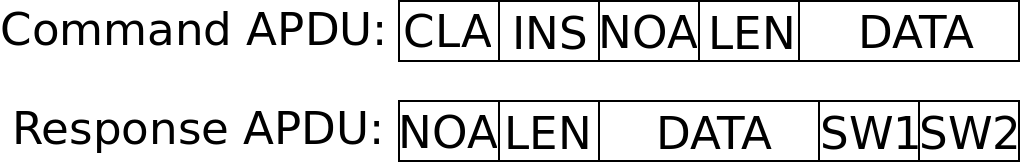
\includegraphics[width=1\hsize]{./images/myapdu.png}
\end{center}
\caption[Selbstdefinierter Dateninhalt der APDUs]{\label{myapdu}Selbstdefinierter Dateninhalt der APDUs}
\end{figure}

%Der Inhalt der APDUs orientiert sich stark an der ISO Norm ISO7816. Der konkrete Aufbau ist in Abbildung apdu.png zusehen (NOA=Number of APDUs)

%Die Modelklassen besitzen Funktionen zur umwandlung zwischen instanzen und byte Arrays zur Übertragung
%diese umwandlung  wurde eigens implementiert und orientiert sich am Aufbau von ethernet Packeten. Ein Packet besteht dabei immer aus einem byte für einen eindeutigen Identifikator, zwei bytes für die anzahl der data bytes sowie bytes für den dateninhalt

%verschlüsselung